% Created 2024-04-08 Mon 21:33
% Intended LaTeX compiler: pdflatex
\documentclass[a4paper, 11pt]{article}
\usepackage[utf8]{inputenc}
\usepackage[T1]{fontenc}
\usepackage{graphicx}
\usepackage{longtable}
\usepackage{wrapfig}
\usepackage{rotating}
\usepackage[normalem]{ulem}
\usepackage{amsmath}
\usepackage{amssymb}
\usepackage{capt-of}
\usepackage{hyperref}
\usepackage{lmodern} % Ensures we have the right font
\usepackage[T1]{fontenc}
\usepackage{inputenc}
\usepackage{graphicx, float}
\usepackage{amsmath, amsfonts, amsthm, amssymb, lipsum}
\usepackage[table, xcdraw]{xcolor}
\usepackage[colorlinks]{hyperref}
\hypersetup{colorlinks, linkcolor=blue, urlcolor=blue}
\setlength{\parindent}{0pt}
\setlength{\parskip}{1em}
\usepackage[stretch=10]{microtype}
\usepackage{hyphenat}
\usepackage{ragged2e}
\usepackage{subfig} % Subfigures (not needed in Org I think)
\usepackage{hyperref} % Links
\usepackage{listings} % Code highlighting
\usepackage[margin=1in, footskip=0.25in]{geometry}
\renewcommand{\baselinestretch}{1.15}
\pagenumbering{gobble}
\usepackage[explicit]{titlesec}
\usepackage{enumitem}
\setlist[itemize]{topsep=0pt}
\newtheorem{theorem}{Theorem}[section]
\newtheorem{corollary}{Corollary}[theorem]
\newtheorem{lemma}[theorem]{Lemma}
\newtheorem{definition}{Definition}[theorem]
\setlength{\abovedisplayskip}{-15pt}
\setlength{\belowdisplayskip}{0pt}
\setlength{\abovedisplayshortskip}{0pt}
\setlength{\belowdisplayshortskip}{0pt}
\author{Bryan Lim Jing Xiang (A0233605M)}
\date{}
\title{Task C}
\hypersetup{
 pdfauthor={Bryan Lim Jing Xiang (A0233605M)},
 pdftitle={Task C},
 pdfkeywords={},
 pdfsubject={},
 pdfcreator={Emacs 29.3 (Org mode 9.7)}, 
 pdflang={English}}
\begin{document}

\maketitle
\section{Dataset}
\label{sec:org970d49b}
\subsection{Overview}
\label{sec:org773d49e}
This dataset consists of CVEs along with their corresponding metrics across the years up to 2023. The data fields of interest are:

\begin{center}
\begin{tabular}{lll}
Field & Description & Data Type\\[0pt]
\hline
cve.published & Name (which denotes month too) & String\\[0pt]
cve.metrics.cvssMetricV31.cvssData.baseSeverity & Severity of CVE & String\\[0pt]
cve.metrics.cvssMetricV31.cvssData.attackVector & Attack Vector of CVE & String\\[0pt]
Year & Year & Integer\\[0pt]
\end{tabular}
\end{center}

Naturally, such a dataset is interesting in view of the recent news over the XZ exploits.
\subsection{Data origin}
\label{sec:orgc84cd51}
\url{https://www.kaggle.com/datasets/manaielyes/cve-vulnerabilities}
\subsection{Github Repository}
\label{sec:org662427b}
\url{https://github.com/bryanljx/visualisation}
\section{Purpose of Visualisation}
\label{sec:orgd32f8f1}
For this dataset, the query of interest is: ``What are current trends/patterns amongst CVEs nowadays? How severe are they and what kind of vulnerabilities are out there?''
\section{Visualisation}
\label{sec:org827b7dc}
\subsection{CVEs per severity category since September 10th, 2019}
\label{sec:orgbbac894}

\begin{center}
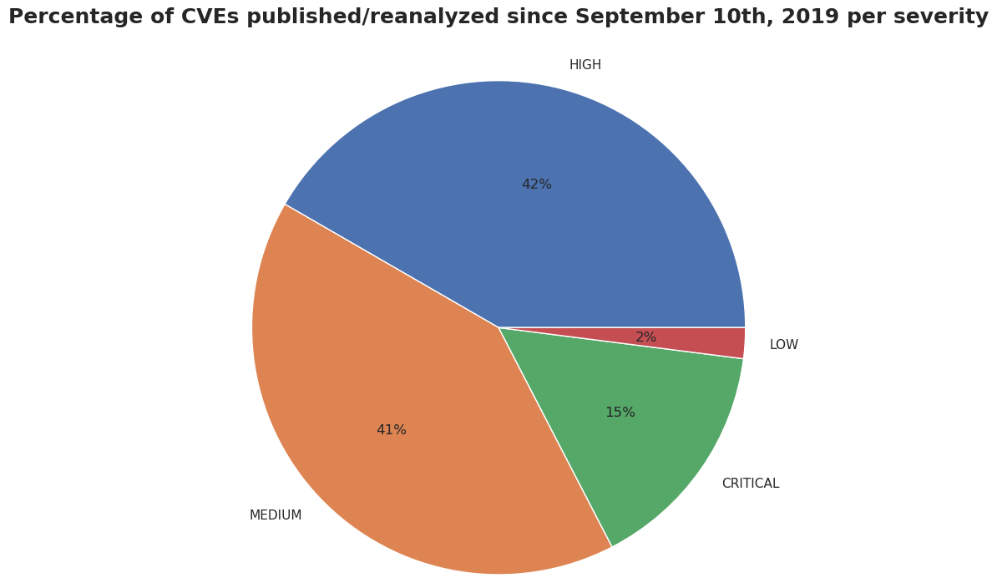
\includegraphics[width=.9\linewidth]{./charts/cve_severity.png}
\end{center}

\begin{itemize}
\item Note: Only data points which have values for the new CVSS v3.1 metric are included, this means only CVEs published after this data or reanalysed after this data are included, which makes for a more recent and current view of CVEs that are of concern today.
\item A pie chart was chosen here to show the distribution of CVEs per severity.
\item Visual encoding here includes:
\begin{itemize}
\item Length - Denoting the percentage of CVEs for each severity
\item Color - Denoting the severity
\end{itemize}
\item Insights
\begin{itemize}
\item Most CVEs are of medium or high severity, with only a select few being critical.
\end{itemize}
\end{itemize}
\subsection{CVEs per attack vector since September 10th, 2019}
\label{sec:org9f3e4ef}

\begin{center}
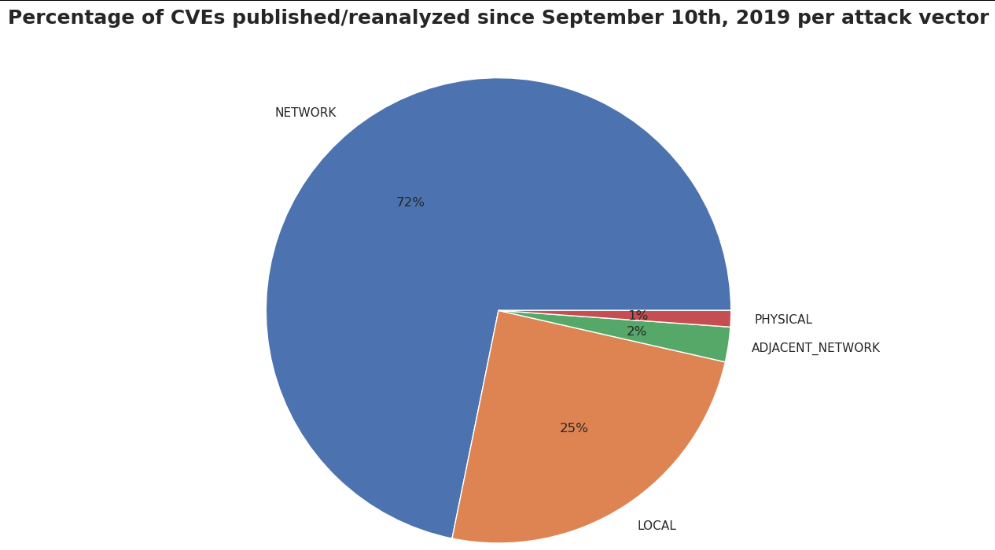
\includegraphics[width=.9\linewidth]{./charts/cve_attack_vector.png}
\end{center}

\begin{itemize}
\item A pie chart was chosen here to show the distribution of CVEs per attack vector.
\item Visual encoding here includes:
\begin{itemize}
\item Length - Denoting the percentage of CVEs for each attack vector
\item Color - Denoting the attack vector
\end{itemize}
\item Insights
\begin{itemize}
\item Network is the most vulnerable attack vector
\end{itemize}
\end{itemize}
\subsection{Distribution of current CVEs across the years}
\label{sec:org7b3991c}

\begin{center}
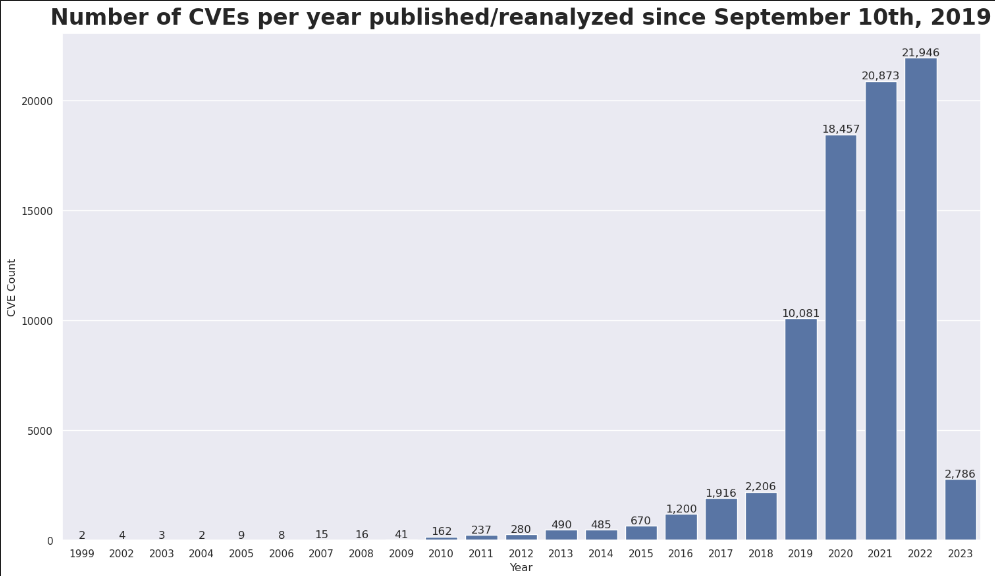
\includegraphics[width=.9\linewidth]{./charts/cve_year.png}
\end{center}

\begin{itemize}
\item A bar chart was chosen to show the number and spread of CVEs still relevant (only those reanalysed or published after September 10th, 2019) across the years
\item Visual encoding here includes:
\begin{itemize}
\item Length: Denoting the number of CVEs published that year still relevant now
\end{itemize}
\item Insights
\begin{itemize}
\item Relatively huge number of CVEs from 2019 - 2022. While this coincides with a greater amount of CVEs reported and published, this may suggest that CVEs are not tackled and resolved that fast, that they are still relevant and a potential attack vector for a few years.
\end{itemize}
\end{itemize}
\end{document}
